%% -*- coding: utf-8 -*-
\documentclass[12pt,a4paper]{scrartcl} 
\usepackage[utf8]{inputenc}
\usepackage[english,russian]{babel}
\usepackage{indentfirst}
\usepackage{misccorr}
\usepackage{graphicx}
\usepackage{amsmath}
\usepackage{changepage}
\usepackage[left=25mm, top=20mm, right=20mm, bottom=20mm, nohead, nofoot]{geometry}
\begin{document}
  \begin{titlepage}
    \begin{center}
      \large
      МИНИСТЕРСТВО НАУКИ И ВЫСШЕГО ОБРАЗОВАНИЯ РОССИЙСКОЙ ФЕДЕРАЦИИ
      
      Федеральное государственное бюджетное образовательное учреждение высшего образования
      
      \textbf{АДЫГЕЙСКИЙ ГОСУДАРСТВЕННЫЙ УНИВЕРСИТЕТ}
      \vspace{0.25cm}
      
      Инженерно-физический факультет
      
      Кафедра автоматизированных систем обработки информации и управления
      \vfill

      \vfill
      
      \textsc{Отчет по практике}\\[5mm]
      
      {\LARGE Создание программы для обработки изображений.}
      \bigskip
      
      2 курс, группа 2ИВТ
    \end{center}
    \vfill
    
    \newlength{\ML}
    \settowidth{\ML}{«\underline{\hspace{0.7cm}}» \underline{\hspace{2cm}}}
    \hfill\begin{minipage}{0.5\textwidth}
      Выполнил:\\
      \underline{\hspace{\ML}} Д.\,Э.~Небольсин\\
      «\underline{\hspace{0.7cm}}» \underline{\hspace{2cm}} 2024 г.
    \end{minipage}%
    \bigskip
    
    \hfill\begin{minipage}{0.5\textwidth}
      Руководитель:\\
      \underline{\hspace{\ML}} С.\,В.~Теплоухов\\
      «\underline{\hspace{0.7cm}}» \underline{\hspace{2cm}} 2024 г.
    \end{minipage}%
    \vfill
    
    \begin{center}
      Майкоп, 2024 г.
    \end{center}
  \end{titlepage}
\label{sec:intro}


\large\tableofcontents

\newpage

\section{Теория}
\subsection{Техническое задание}
\textbf {Задание:}

Создать программу для обработки изображений, которая будет выполнять следующие функции: изменение яркости, контрастности и насыщенности цветов.

\subsection{Теоретическая часть} 

Яркость изображения - это мера светимости или интенсивности света, которую излучает или отражает изображение. Она определяет, насколько ярким или темным выглядит изображение. Она зависит от различных факторов, включая освещение сцены, контрастность, цветовую гамму и настройки яркости на устройстве воспроизведения. Увеличение яркости может сделать изображение более четким и легкочитаемым, но слишком высокая яркость может привести к искажению цветов и потере деталей.\textit{}

Контраст - это разница в яркости и/или цвете, которая делает объект различимым. В визуальном восприятии реального мира, контрастность определяется разницей в цвете и яркости объекта и других объектов в пределах одного и того же поля зрения. Поскольку человеческая зрительная система является более чувствительной к контрасту в абсолютной яркости, мы можем воспринимать мир аналогично, независимо от изменений освещения в течение суток или от места к месту. Максимальный контраст изображения зависит от контрастного коэффициента и динамического диапазона.\textit{}

Насыщенность, которую также называют «интенсивностью цвета», описывает силу цвета относительно его яркости или светлоты. Иными словами, насыщенность цвета обозначает его отличие от серого при определённой яркости освещения. Например, цвета близкие к серому ненасыщенные по сравнению с более светлыми цветами.

\newpage

\section{Ход работы}
\label{sec:exp}

\subsection{Код приложения}
\label{sec:exp:code}
\begin{verbatim}
<!DOCTYPE html>
<html lang="en">
<head>
    <meta charset="UTF-8">
    <meta name="viewport" content="width=device-width,
                initial-scale=1.0">
    <title>Обработка изображения</title>
    <style>
        #image{
            width: 25%;
            padding: 10px;
            margin: 10px;
            border: 2px solid;
        }
        .sliderContainer {
            width: 25%;
            display: flex;
            flex-direction: row;
            gap: 10px;
        }
        .slider {
            width: 200px;
        }
        h3 {
            width: 200px;
        }
    </style>
</head>
<body>
    <h1>Обработка изображения</h1>
    <h3>Учебная практика</h3>
    <div>
        <p><input type="file" id="imageFile" 
                    onchange="loadImage(event)"></p>
        <img id="image" src="" alt="Изображение">
    </div>

    <div class="sliderContainer">
        <h3>Насыщенность</h3>
        <input type="range" min="0" max="200" 
                    value="100" class="slider" id="saturate">
        <h3 id="saturateValue"></h3>
    </div>

    <div class="sliderContainer">
        <h3>Контраст</h3>
        <input type="range" min="0" max="200" 
                    value="100" class="slider" id="contrast">
        <h3 id="contrastValue"></h3>
    </div>

    <div class="sliderContainer">
        <h3>Яркость</h3>
        <input type="range" min="0" max="200" 
                    value="100" class="slider" id="brightness">
        <h3 id="brightnessValue"></h3>
    </div>

    <input type="button" onclick="saveImage()" 
                    value="Сохранить изображение">

    <input type="button" onclick="resetSliders()" 
                    value="Сбросить фильтры">

    <script>
        const image = document.getElementById('image');

        const sliderSaturate = document.getElementById("saturate");
        const sliderSaturateValue = 
                    document.getElementById("saturateValue");
        sliderSaturateValue.innerHTML = sliderSaturate.value + '%';
        sliderSaturate.oninput = function() {
            sliderSaturateValue.innerHTML = this.value + '%';
            image.style.filter = getFilter();
        }

        const sliderContrast = document.getElementById("contrast");
        const sliderContrastValue = 
                    document.getElementById("contrastValue");
        sliderContrastValue.innerHTML = sliderContrast.value + '%';
        sliderContrast.oninput = function() {
            sliderContrastValue.innerHTML = this.value + '%';
            image.style.filter = getFilter();
        }

        const sliderBrightness = document.getElementById("brightness");
        const sliderBrightnessValue = 
                    document.getElementById("brightnessValue");
        sliderBrightnessValue.innerHTML = sliderBrightness.value + '%';
        sliderBrightness.oninput = function() {
            sliderBrightnessValue.innerHTML = this.value + '%';
            image.style.filter = getFilter();
        }

        function loadImage(event) {
            var reader = new FileReader();
            reader.onload = function() {
                image.src = reader.result;
            }
            reader.readAsDataURL(event.target.files[0]);
        }

        function saveImage() {    
            const canvas = document.createElement('canvas');
            const context = canvas.getContext('2d');
            canvas.width = image.width;
            canvas.height = image.height;
            context.filter = getFilter();
            context.drawImage(image, 0, 0, image.width, image.height);
            const dataURL = canvas.toDataURL('image/jpeg');

            const link = document.createElement('a');
            link.href = dataURL;
            link.download = 'modified_image.jpg';
            link.click();
        }

        function resetSliders() {
            sliderSaturateValue.innerHTML = 100;
            sliderSaturate.value = 100;
            sliderContrastValue.innerHTML = 100;
            sliderContrast.value = 100;
            sliderBrightnessValue.innerHTML = 100;
            sliderBrightness.value = 100;
            image.style.filter = getFilter();
        }

        function getFilter() {
            return `
                brightness(${sliderBrightness.value}%) 
                contrast(${sliderContrast.value}%) 
                saturate(${sliderSaturate.value}%)`
        }

    </script>
</body>
</html>
\end{verbatim}

\subsection{Работа программы}


\begin{wrapfigure}
  \begin{center}
    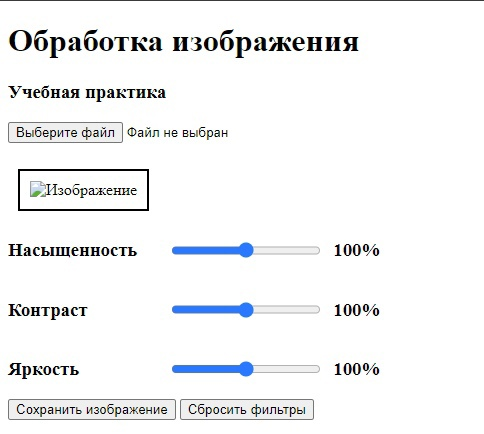
\includegraphics[width=0.40\textwidth]{ui.jpg}
  \end{center}
  \caption{Рис.1  Внешний вид интерфейса}\label{fig:ex}
\end{wrapfigure}

\begin{wrapfigure}
  \begin{center}
    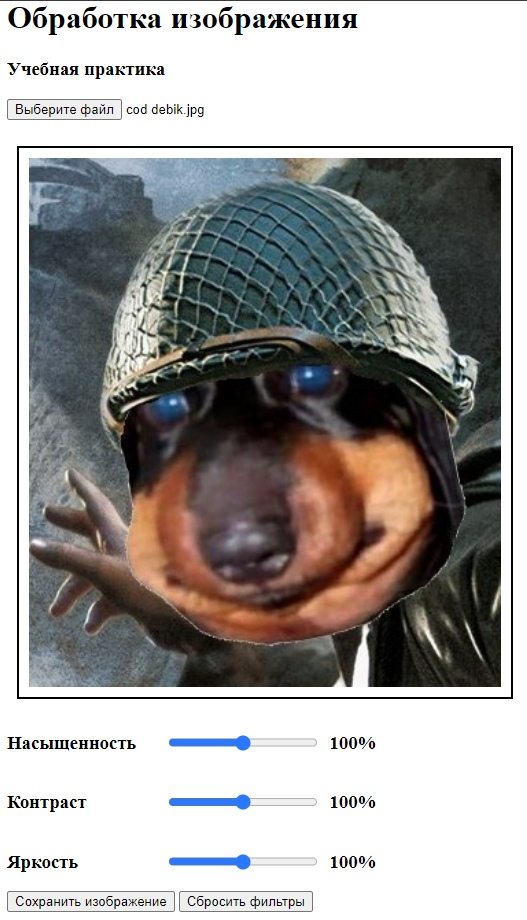
\includegraphics[width=0.36\textwidth]{primer0.jpg}
  \end{center}
  \caption{Рис.2  Изображение до обработки}\label{fig:ex}
\end{wrapfigure}

\begin{wrapfigure}
  \begin{center}
    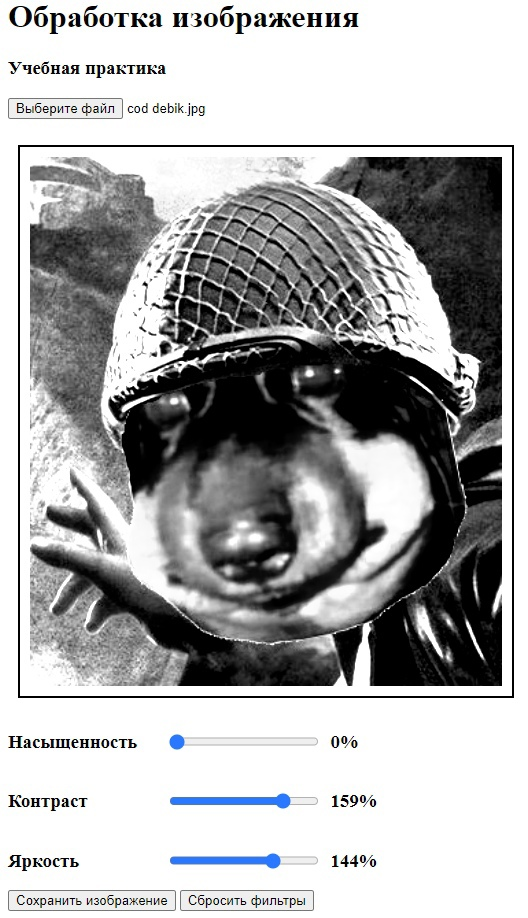
\includegraphics[width=0.36\textwidth]{primer1.jpg}
  \end{center}
  \caption{Рис.2  Пример обработки изображения}\label{fig:ex}
\end{wrapfigure}

\begin{wrapfigure}
  \begin{center}
    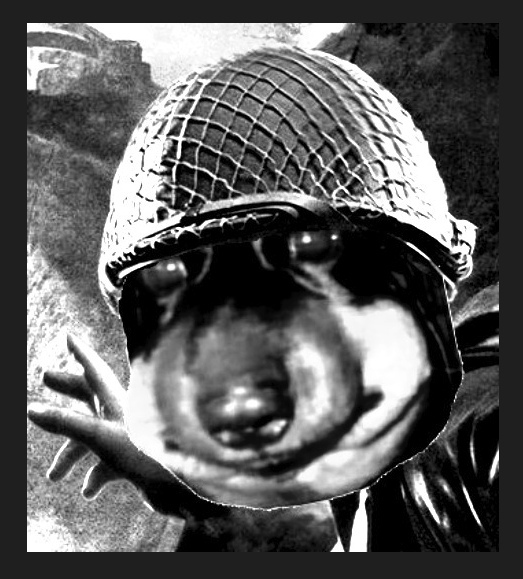
\includegraphics[width=0.5\textwidth]{primer2.jpg}
  \end{center}
  \caption{Рис.3  Итоговое изображение}\label{fig:ex}
\end{wrapfigure}

\end{document}
